\section{The LHCb detector}

LHCb is a particle detector with the main focus on decays in which $b$ or $c$ quarks are involved.
Its goals are precision measurements on the CP-violation and on rare decays. 
To accomplish this it has been build as a single arm forward-spectrometer covering angles to the beam pipe from $\qty{10}{\milli\radian}$ to $\qty{300}{\milli\radian}$ \cite{LHCb}. 
This is because the majority of high energetic $b$-/$c$-hadron pairs, produced in $pp$ collisions, have velocities in roughly the same direction as one of the incident protons.
An overview of the detector is shown in \autoref{fig:lhcb_detector}.
The following paragraphs briefly describe the components of the LHCb detector based on the article \enquote{The LHCb Detector at the LHC}\cite{LHCb}.

\begin{figure}
    \centering
    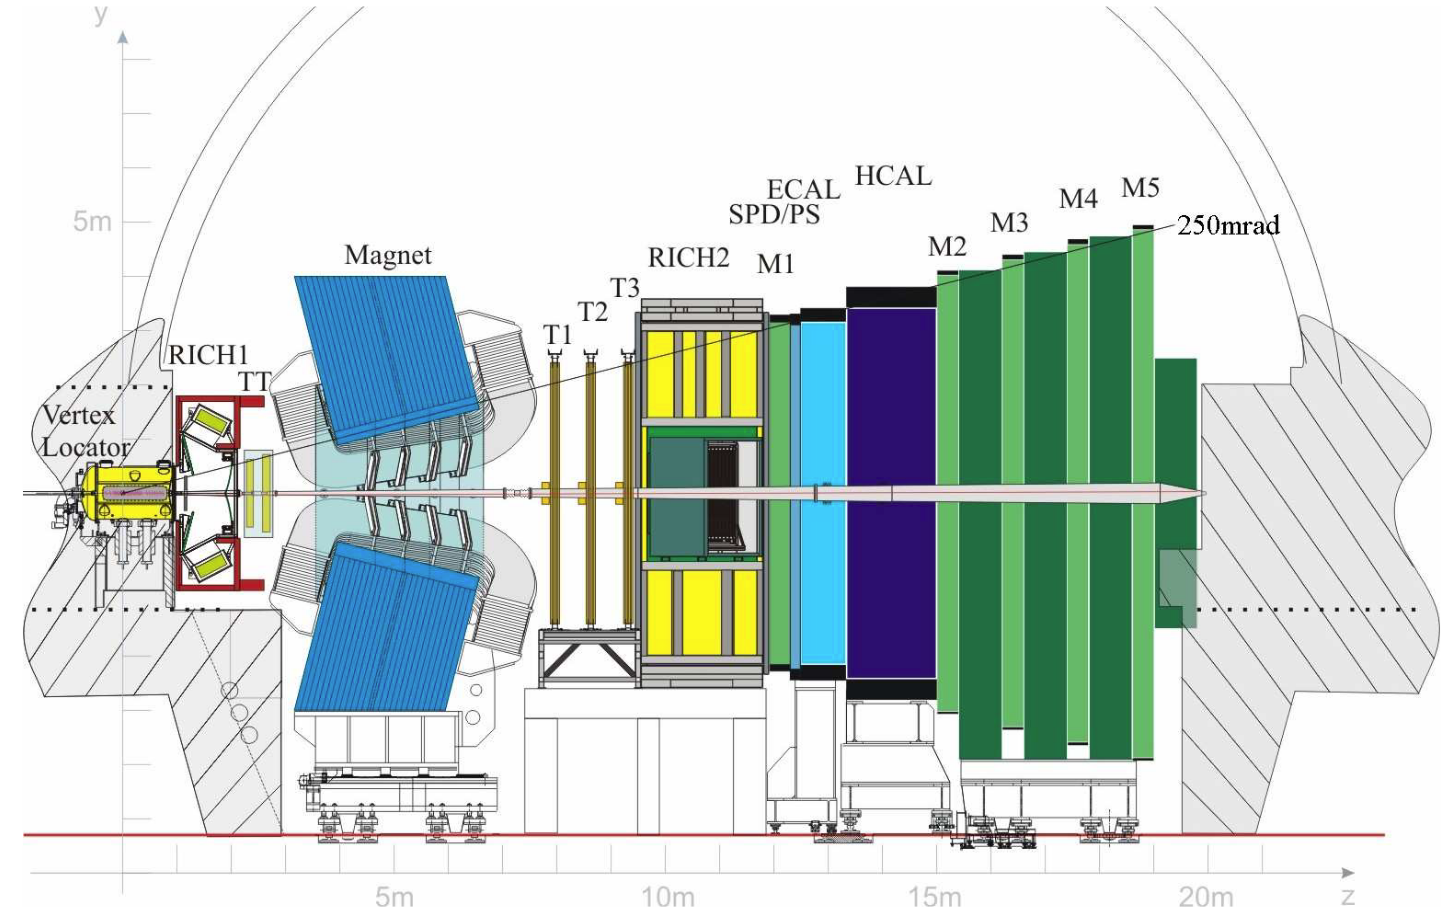
\includegraphics[width=\textwidth]{images/lhcb_detector.png}
    \caption{View of the LHCb detector \cite{LHCb}. }
    \label{fig:lhcb_detector}
\end{figure}

A particle produced at the primary vertex first traverses the Vertex Locator (VELO). 
There, the tracks of charged particles are measured using silicon semiconductor sensors. 
This information then is primarily used to reconstruct the position of the primary and secondary vertices of the decay particles.

Beyond the VELO, the Tracking System then further measures the position over time of the same particles. 
This is done in the Tracker Turicensis (TT) before the magnet and in the Trackers T1, T2 and T3 behind the magnet.
The dipole magnet bends the particle tracks so that the particles' momentum can be inferred.
While the TT and the inner parts of the T1-T3 also use silicon semiconductor sensors, the outer parts of the T1-T3 use scintillating fibre detectors.

The Ring Imaging Cherenkov detectors (RICH1, RICH2) are used to measure the velocities of the particles.
By traversing optically dense materials, charged particles induce the emission of Cherenkov radiation.
This radiation is then detected using photo multipliers and its opening angle is closely related to the velocity of a particle.

The calorimeters (SPD/PS, ECAL, HCAL) stop most particles and measure their energy.
In dense materials particles induce particle showers with its size directly related to the energy deposited.
Each calorimeter is structured in alternating layers of absorbers and scintillators.
The electronic calorimeter (ECAL) absorbs electrons, positrons and photons, and the hadronic calorimeter (HCAL) absorbs any hadrons.
These are the only detectors at LHCb which can detect chargeless particles, and they are critical for particle identification.

To identify particles as muons the muon chambers (M1-M5) stop and track charged particles which pass through the calorimeters without absorption.
They use iron layers to stop the muons and multi-wire proportional chambers to detect them.

The only known particles that pass through the LHCb detector undetected are neutrinos.
They are indirectly measured through analysis of the missing transversal momentum and energy. 


